
\chapter{Introduction}

\minitoc

One fundamental goal of Artificial Intelligence (\ai) is to design embodied autonomous interactive agents that can evolve in various environments and complete a wide range of tasks. To that end, researchers in \ai take several angles of attack and rely on different paradigms that consider different drivers for learning. 
\begin{itemize}[noitemsep]
\item In Reinforcement Learning (\rl)~\citep{sutton2018reinforcement}, agents learn from \textit{exploration} of their environment. They rely solely on their experience of the world in order to solve a pre-defined task. 
\item In Imitation Learning (\il)~\citep{pomerleau1991efficient}, agents learn from \textit{demonstrations}, i.e. trajectories provided by an expert that correspond to the transitions required to take in order to solve a pre-defined task. 
\item In Multi-Agent Learning~\citep{LITTMAN1994157}, agents learn in \textit{cooperation} and need to interact with each other in order to solve collaborative tasks.
\end{itemize}

Recent extensions of \rl algorithm have shown success in solving a wealth of problems such as playing the Atari videogames at super-human levels~\citep{mnih2015human}, beating chess and go world champions~\citep{silver2016mastering}, controlling stratospheric baloons~\citep{bellemare2020autonomous} or even maintaining plasma in fusion reactors~\citep{degrave2022magnetic}. Similarly, \il methods coupled to Transformers~\citep{vaswani2017attention} have enabled the training of a generalist agent on a massive dataset of diverse interactions~\citep{reed2022a}. It has also been used to perform in-context reinforcement learning via algorithm distillation~\citep{laskin2022incontext}. Finally, multi-agent methods have permitted populations of agents to play hide and seek~\citep{Baker2020Emergent} or even to collaboratively solve common-pool resource problems~\citep{perolat2017commonpool}.

But unlike humans, these algorithms are still heavily sample-inefficient, requiring billions of transitions to become proficient on isolated tasks. Crucially, they lack the ability to generalize and transfer across a wide variety of problems. This is, perhaps, because they rely on isolated signals for learning. The way forward might be to build on child development theory and to consider learning from \textit{socio-cultural interactions}.

\section{Humans are goal-directed social learners}

\paragraph{Humans are autotelic learners}

\paragraph{Humans are social learners}

Humans are social beings; intrinsically motivated to interact and cooperate with their peers~\citep{tomasello_cultural_1999,tomasello_understanding_2005, brewer2014addressing}. Most of our skills could not be learned in isolation. Formal education teaches us to reason systematically, books teach us history, and YouTube might teach us how to cook. Most importantly, our values, traditions, norms and most of our goals are cultural in essence.

This knowledge, and some argue, some of our highest cognitive functions such as abstraction, compositional imagination or relational thinking, are formed through linguistic and cultural interactions with others

 For Vygotsky, linguistic social interactions such as descriptions, explanations, corrections, or play start as interpersonal processes before they are turned into intrapersonal cognitive processes through the process of internalization. 33–35 Following his vision, many psychologists,36–38 linguists,39–41 and philosophers42–45 argued for the importance of socio-cultural interactions in the development of human intelligence.


\section{Towards Interactive Social Autonomous Agents}

Not necessarily a shift of paradigm but rather using social interactions (language and culture rachets) inside previous paradigms:

\begin{figure}[!h]
\centering
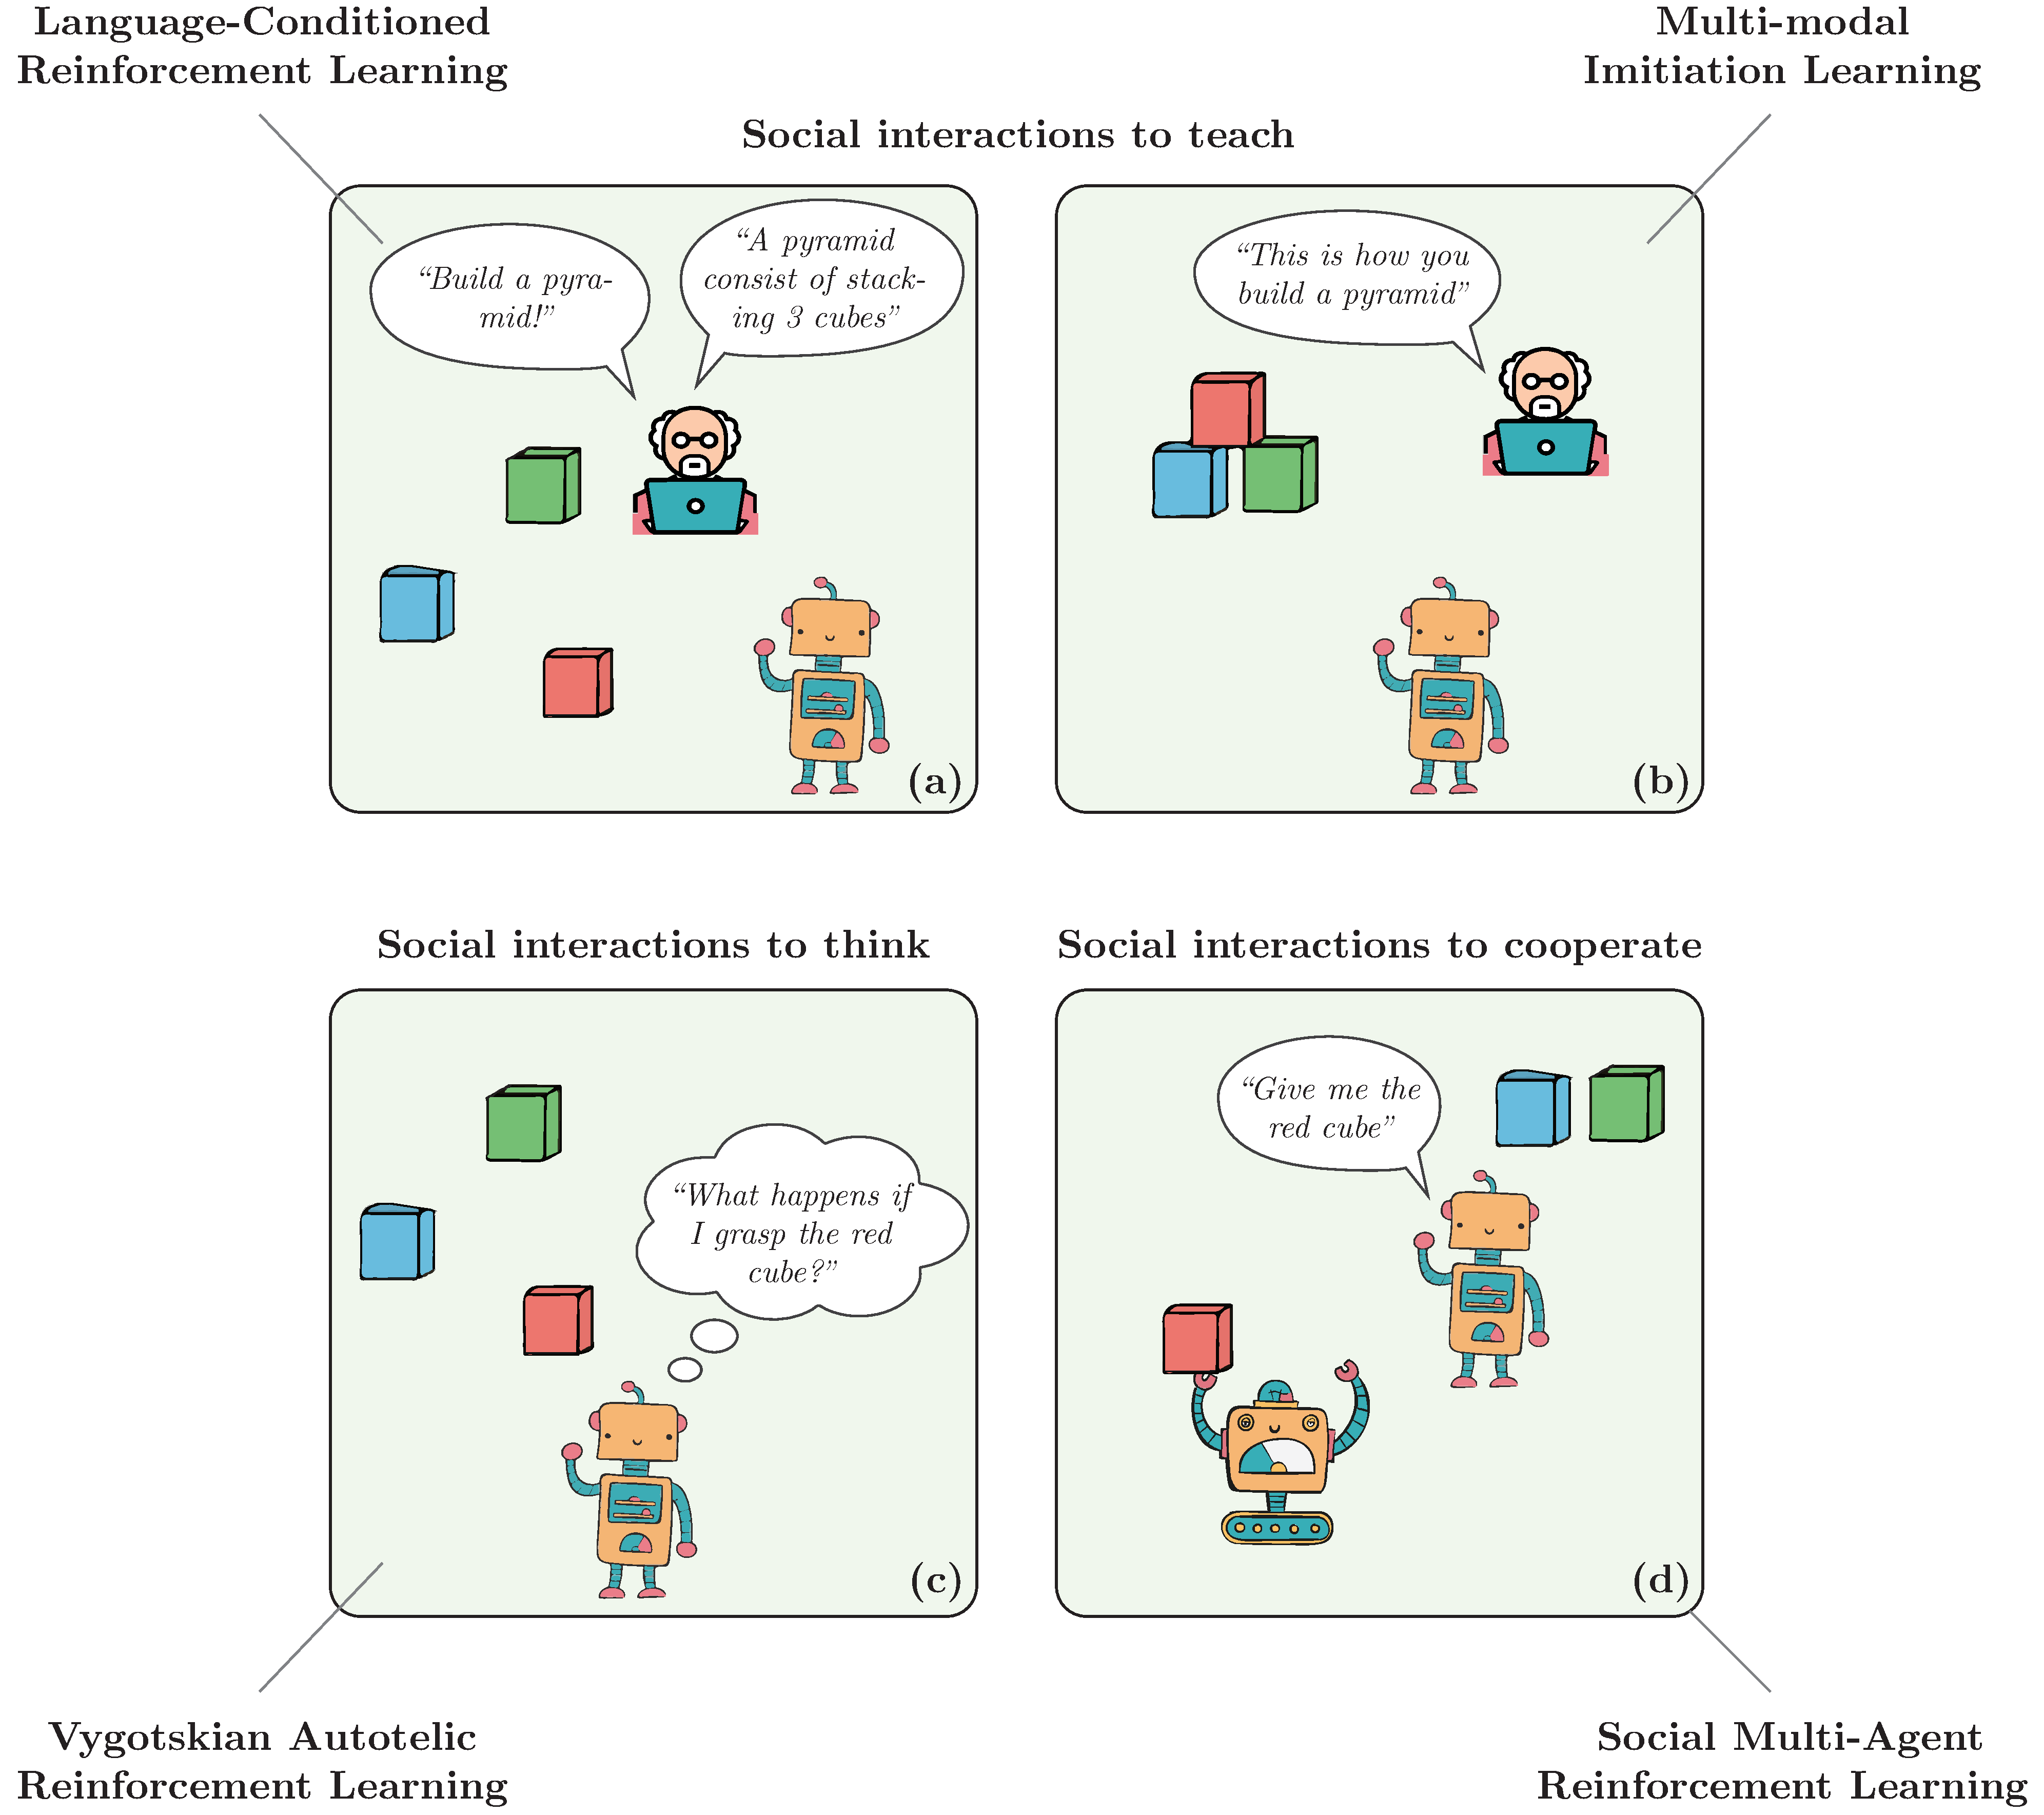
\includegraphics[width=1\textwidth]{intro/language_paradigms.pdf}
\caption{}
\label{fig:intro_language_paradimgs}
\end{figure}

Inside social interaction is language and culture rachets they can be used to:
\begin{itemize}[noitemsep]
\item Language to cooperate
\item Language to teach \cite{sigaud2021towards}
\item Language to organize thoughts	
\end{itemize}


\paragraph{Objectives and Contributions}

This manuscript is organized around two main questions:
%
\begin{enumerate}[noitemsep]
	\item How can such a cultural model emerge in populations of agents?
	\item How can agents leverage existing cultural models to become better learners? 
\end{enumerate}

There is no open-endedness without culture. From an engineering perspective, building open-ended environments for artificial agents requires a community effort.

Culture as youtube videos (from perspective)

Citation (bruner, vygotsky)

\clearpage

\paragraph{Chronological order of publications}

\paragraph{Collaborations}



